\chapter{Conclusion and Future Work} \label{chap4}

\section{Introduction}

In this chapter, we outline the directions of our future research on
non-determinism and its impact on reproducibility of HPC applications.
So far, we have discussed the numerical challenge of reproducibility
in HPC separately from the debugging challenge; work in progress seeks
to establish connections between the two problems and their
solutions. To this end, in future work we will study connections
between run-to-run numerical variability in large scale applications
(as explored in Chapter~\ref{chap2}) and non-deterministic
communication patterns identified with record-and-replay tools (as
explored in Chapter~\ref{chap3}). The study and generalization of
non-deterministic communication patterns not only addresses
un-answered questions that were raised in the previous chapter, but
also provides a platform for identifying code motifs in applications
that lack in numerical reproducibility. We will build our work on
non-deterministic communication patterns on top of preliminary
findings from our attempts to attribute out-of-order receives to
particular communication patterns in MCB described in the next
section. The non-determinism in communication patterns cannot be
addressed without the development of better ticking policies that
mitigate the number of out-of-order events in HPC
applications. Therefore we will look at strategies to improve the
results presented in Chapter~\ref{chap3}.

\section{Out-of-Order Events and Communication Patterns}

In Chapter~\ref{chap3} we investigate the overall rate of out-of-order
messages originating from any of three communication patterns in MCB
(i.e., the neighbor-to-neighbor particle exchange, the non-blocking
gather, and the non-blocking scatter in
Figure~\ref{fig:mcb_comm_patterns}). In this section, we refine our
perspective by presenting data on the messages exchanged between
particular pairs of processes which, combined with knowledge of which
processes receive from which others during each communication pattern,
provides insight into which communication patterns are responsible for
the majority of out-of-order message receives.

To capture the specific senders of out-of-order messages to each
receiving process for each communication pattern, we instrumented the
ReMPI code to write to a log file for each received message. Note that
the log file is separate from the actual record file generated for
ReMPI use during replay. We repeated the tests described in
Figure~\ref{fig:parameter_matrix}. For each of the four cells in
Figure~\ref{fig:parameter_matrix}, we built a first heatmap with total
number of messages and a second heatmap with the total out-of-order
messages.  Specifically, in the first heatmap, for each receiving
process on the row of the heatmap, we collected the total number of
messages this process receives from each sending process on the
columns of the heatmap; the second heatmap is built in the same way
but with the number of out-of-order messages. The intensity of a
cell's coloring in the two heatmaps indicates the number of
messages. Cells colored grey indicate that no messages are
communicated between the process on the cell's row (receiving process)
and the process on the cell's column (sending process).
\begin{figure}[!htb]
    \centering
    \includegraphics[width=\linewidth]{chapter_3_figures/heatmap_interpretation}
    \caption{Interpreting a heatmap of message receives. The receiving
      processes are listed per row; the sending processes are listed
      per column.}
    \label{fig:heatmap_interpretation}
\end{figure}

Figure~\ref{fig:heatmaps_total} shows the total number of messages
received by each receiving process from each process that sent to
it. This data is collected from a 1-node, 16-process run of MCB which
was recorded using ReMPI with MPI\_SEND-ticking (the best of the two
replayable record-and replay techniques in
Chapter~\ref{chap3}. Figure~\ref{fig:heatmaps_total}.(a) refer to high
communication intensity with low floating-point workload (i.e., 1K
particles per process with a buffer size of 5);
Figure~\ref{fig:heatmaps_total}.(b) refers to low communication
intensity with low floating point workload (i.e., 1K particles per
process with a buffer size of 5K); Figure~\ref{fig:heatmaps_total}.(c)
refers to low communication intensity with high floating-point
workload (i.e., 1M particles per process, with a buffer size of 5);
and Figure~\ref{fig:heatmaps_total}.(d) refers to high communication
intensity with low floating-point workload (i.e., 1M particles per
process, with a buffer size of 5K).
\begin{figure}[ht!]
    \begin{minipage}[b]{0.5\linewidth}
        \centering
     \includegraphics[width=0.95\linewidth]{chapter_3_figures/heatmap_total_nodes1_procs16_cycles10_particles1000_bufferSize5}
        \\ (a) \\ 
    \end{minipage}%
    \begin{minipage}[b]{0.5\linewidth}
        \centering
     \includegraphics[width=0.95\linewidth]{chapter_3_figures/heatmap_total_nodes1_procs16_cycles10_particles1000_bufferSize5000}
       \\ (b) \\
    \end{minipage}
    \begin{minipage}[b]{0.5\linewidth}
        \centering
        \includegraphics[width=0.95\linewidth]{chapter_3_figures/heatmap_total_nodes1_procs16_cycles10_particles1000000_bufferSize5}
       \\ (c) \\
    \end{minipage}%
    \begin{minipage}[b]{0.5\linewidth}
        \centering
        \includegraphics[width=0.95\linewidth]{chapter_3_figures/heatmap_total_nodes1_procs16_cycles10_particles1000000_bufferSize5000}
       \\ (d) \\
    \end{minipage}
    \caption{Total number of messages received by each receiving
      process $i$ per sender process $j$ for a testcase of 1K
      particles per process, buffer size 5 (a); 1K particles per
      process, buffer size 5K (b); 1M particles per process, buffer
      size 5 (c); and 1M particles per process, buffer size 5K (d).}
    \label{fig:heatmaps_total}
\end{figure}

Figure~\ref{fig:heatmaps_out_of_order} shows heatmaps counting only
the out-of-order receives. This data is a subset of that shown in
Figure~\ref{fig:heatmaps_total} and refers to the same four
communication intensity and floating-point workload scenarios studied
above.
\begin{figure}[ht!]
    \begin{minipage}[b]{0.5\linewidth}
        \centering
        \includegraphics[width=0.95\linewidth]{chapter_3_figures/heatmap_out_of_order_nodes1_procs16_cycles10_particles1000_bufferSize5}
        \\ (a) \\
    \end{minipage}%
    \begin{minipage}[b]{0.5\linewidth}
        \centering
        \includegraphics[width=0.95\linewidth]{chapter_3_figures/heatmap_out_of_order_nodes1_procs16_cycles10_particles1000_bufferSize5000}
       \\ (b) \\
    \end{minipage}
    \begin{minipage}[b]{0.5\linewidth}
        \centering
        \includegraphics[width=0.95\linewidth]{chapter_3_figures/heatmap_out_of_order_nodes1_procs16_cycles10_particles1000000_bufferSize5}
       \\ (c) \\
    \end{minipage}%
    \begin{minipage}[b]{0.5\linewidth}
        \centering
        \includegraphics[width=0.95\linewidth]{chapter_3_figures/heatmap_out_of_order_nodes1_procs16_cycles10_particles1000000_bufferSize5000}
      \\ (d) \\ 
    \end{minipage}
    \caption{Total number of out-of-order messages received by each receiving
      process $i$ per sender process $j$ for a test case of 1K
      particles per process, buffer size 5 (a); 1K particles per
      process, buffer size 5K (b); 1M particles per process, buffer
      size 5 (c); and 1M particles per process, buffer size 5K (d).}
    \label{fig:heatmaps_out_of_order}
\end{figure}

The heatmaps with the total number of communicated message in
Figure~\ref{fig:heatmaps_total} outline how some processes only
receive from some other processes during certain communication
patterns. For example, process $P_0$ does not receive messages from
process $P_2$ during the neighbor-to-neighbor particle exchange, but
does receive messages from process $P_2$ during the nonblocking
gather. The four heatmaps in the figure confirm the three
communication patterns that we had previously extracted with the
manual inspection of the MCB code in
Figure~\ref{fig:mcb_comm_patterns}.

The inspection of the heatmaps of out-of-order messages outline which
one, if any, of the three communication patterns impacts the
non-determinism the most. In Figure~\ref{fig:heatmaps_out_of_order} we
observe that the nonblocking gather pattern is responsible for a
disproportionate amount of the out-of-order messages received. In
Figure~\ref{fig:comm_patterns_fault}, we highlight cells of the
heatmaps to indicate attribution of out-of-order receives to
particular communication patterns. Once again we observe that cells
indicating the greatest number of out-of-order receives correspond to
messages sent during the non-blocking gather communication pattern,
whereas the non-blocking scatter pattern exhibits the least.
\begin{figure}
    \centering
    %\includegraphics[width=\linewidth]{chapter_3_figures/comm_patterns_fault}
    \begin{minipage}[b]{0.33\linewidth}
        \centering
        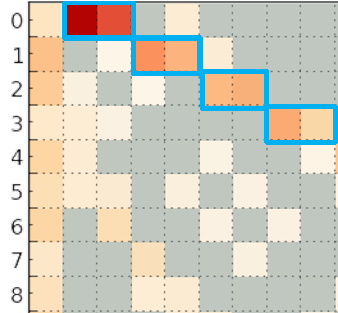
\includegraphics[width=0.9\linewidth]{chapter_4_figures/partial_heatmap_total_gather}
    \end{minipage}%
    \begin{minipage}[b]{0.33\linewidth}
        \centering
        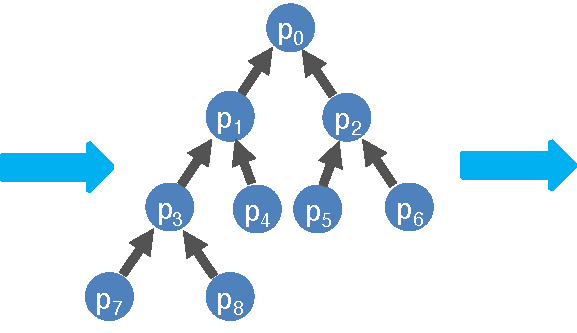
\includegraphics[width=\linewidth]{chapter_4_figures/comm_pattern_gather}
    \end{minipage}%
    \begin{minipage}[b]{0.33\linewidth}
        \centering
        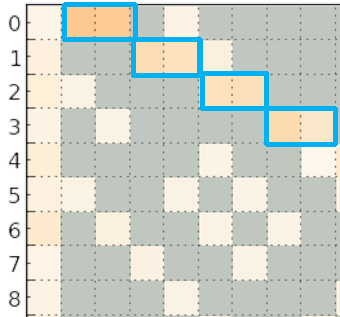
\includegraphics[width=0.9\linewidth]{chapter_4_figures/partial_heatmap_out_of_order_gather}
    \end{minipage}
    \\
    \begin{minipage}[b]{0.33\linewidth}
        \centering
        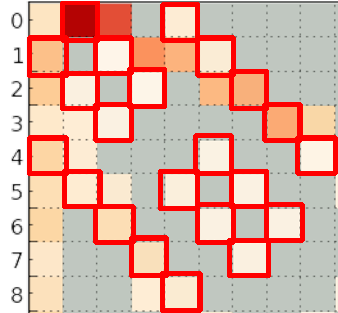
\includegraphics[width=0.9\linewidth]{chapter_4_figures/partial_heatmap_total_n2n}
    \end{minipage}%
    \begin{minipage}[b]{0.33\linewidth}
        \centering
        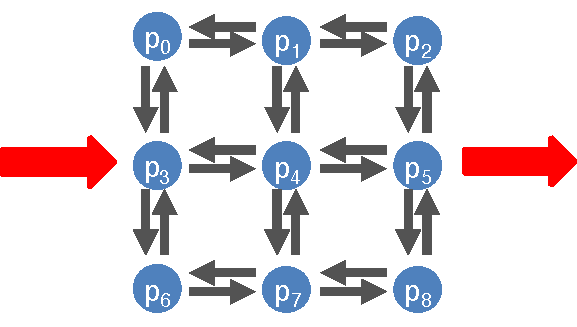
\includegraphics[width=\linewidth]{chapter_4_figures/comm_pattern_n2n}
    \end{minipage}%
    \begin{minipage}[b]{0.33\linewidth}
        \centering
        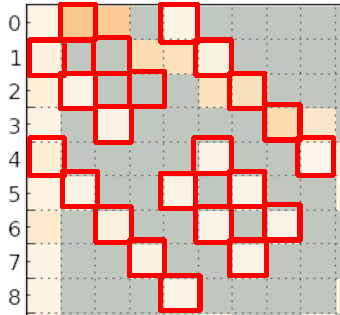
\includegraphics[width=0.9\linewidth]{chapter_4_figures/partial_heatmap_out_of_order_n2n}
    \end{minipage}
    \\
    \begin{minipage}[b]{0.33\linewidth}
        \centering
        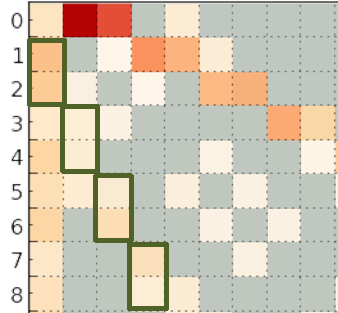
\includegraphics[width=0.9\linewidth]{chapter_4_figures/partial_heatmap_total_scatter}
        \\ (a) \\
    \end{minipage}%
    \begin{minipage}[b]{0.33\linewidth}
        \centering
        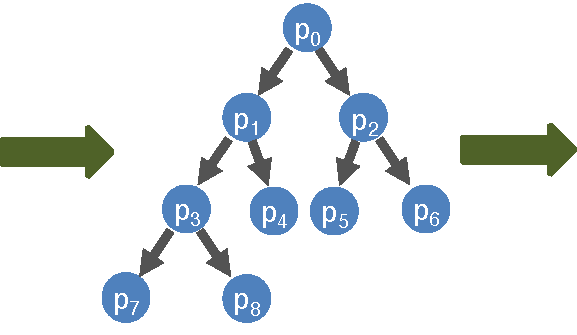
\includegraphics[width=\linewidth]{chapter_4_figures/comm_pattern_scatter}
        \\ (b) \\
    \end{minipage}%
    \begin{minipage}[b]{0.33\linewidth}
        \centering
        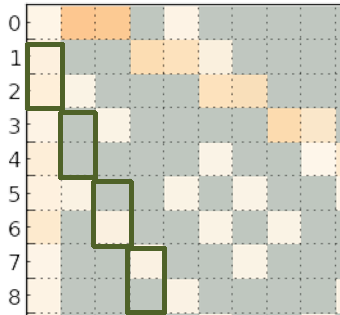
\includegraphics[width=0.9\linewidth]{chapter_4_figures/partial_heatmap_out_of_order_scatter}
        \\ (c) \\
    \end{minipage}
    \caption{Linking out-of-order receives to one of the three MCB
      communication patterns presented in
      Figure~\ref{fig:mcb_comm_patterns}. Because of space constraints
      only a quarter of each heatmap is shown.
      Each row shows heatmaps with receiving processes highlighted that participate in a given communication pattern.
      Column (a) shows heatmaps of total number of receives;
      column (b) shows the communication pattern;
      and column (c) shows heatmaps of the number of out-of-order receives.}
    \label{fig:comm_patterns_fault}
\end{figure}
These results are a first insight in the impact of single
communication patters on non-determinism.

\section{Adaptive Ticking Policies}

Our observation that particular out-of-order receives can be
attributed to particular communication patterns suggests a general
technique for improving a ticking policy. We propose to develop an
\textit{adaptive ticking policy} that is based on application-level
events such as floating-point instructions, but also takes into
account processes' placement in the communication topology and the
phase of communication the application is currently engaged. Our
future work in on adaptive ticking policies will proceed along two
branches.

We will first expand our investigation of communication
patterns that are found in non-deterministic HPC applications, and
enrich our understanding of how these communication patterns interact,
specifically, with ticking policies, and more generally, with record
and replay tools. We will progress this line of research by
identifying non-deterministic communication patterns in real
applications, modeling their critical characteristics, and developing
microbenchmarks based on these patterns so that their responses to
ticking policies and record-and-replay tools can be studied in
isolation. By doing so, we will systematize adaptation of tools to
applications.

Second, we will investigate the feasibility of enhancing ticking
policies such as our FLOPs-ticking with high-level information about
application behavior, such as what kind of communication pattern the
application is currently engaged in. Since we have shown that a
ticking policy that works well in one scenario (e.g., low
communication intensity and low floating-point workload) may not offer
the same benefits in another scenario, it behooves us to investigate
the feasibility of ticking policies that can adapt to application
characteristics on the fly.

%\section{Alternative Encoding of the Matched-Test Table} A
%fundamental problem that is addressed by CDC is how to represent the
%permutation that maps the observed message receive order to the
%logical clock reference order. CDC opts to represent the permutation
%by a table of indices and offsets which effectively describe the
%\textit{edits} determined by the CDC edit distance algorithm. To the
%best of our knowledge there does not exist a proof that this
%representation has minimum size for all permutations on the set of
%observed messages. Hence, we will investigate alternative encoding
%strategies for the permutations that the matched-test table must
%encode.  One alternative for representing permutations is by
%permutation ranking. Give a set of $n$ elements, it is possible to
%impose a total order on the $n!$ permutations of that set. In fact,
%one can impose one of many distinct totals orders upon that set of
%permutations. Once such a total order is imposed, one can represent a
%permutation $p$ by its rank--i.e., a single integer in the range
%$\{0, \ldots, n!\}$. While such integers, even for small $n$, can
%exceed the capacity of a 64-bit unsigned integer to represent and as
%such necessitate an arbitrary precision arithmetic library, there
%exist fast algorithms for computing the rank of a permutation
%~\cite{PermutationRanking:Myrvold:2001} and as such it may be
%worthwhile to compute permutation ranks in the event that that
%representation offers a significant reduction in size relative to the
%CDC table Another promising encoding technique for general
%permutations is proposed by Barbay and Navarro in their work on
%\textit{Left-to-Right-Minima Trees} (LRM Trees)\cite{}. This work
%describes a compressed data structure for representing permutations
%compactly that also enables a fast algorithm for application of the
%permutation, which CDC must do during replay. In particular, the
%compressed data structure enables the application of the permutation
%without decompression.

\section{Investigating Numerical Irreproducibility via Record-and-replay}

In addition to gleaning insight into how patterns of non-deterministic
communication impact the cost of applying record-and-replay techniques
such as CDC, our efforts to develop a taxonomy of non-deterministic
communication patterns will provide insight into how numerical
accuracy is impacted by non-deterministic communication. Specifically,
the ordering of receives in message-passing applications impacts
numerical reproducibility of those applications when variability in
message arrivals re-orders floating-point operands. We will explore
the use of record-and-replay tools for capturing executions exhibiting
highly accurate results, as well as those exhibiting highly inaccurate
results, in order to ascertain the internal properties of those
executions that induced, respectively, accuracy or inaccuracy.

\section{Summary}

In this thesis, we tackled the dual challenges of loss of numerical
reproducibility and loss of debuggability that non-determinism in HPC
applications presents. In response to the numerical challenge we
presented a strong case for selection of summation algorithms based on
characteristics of the floating-point operands an application is
likely deal with, and showed a quantitative comparison of compensated
summation algorithms' responses to the dynamic range and conditioning
of their inputs. 

In response to the debugging challenge, we investigated a fine-grained
logical clock ticking policy based on floating-point operations for
use in the Clock-Delta Compression record-and-replay
technique. Although our ticking policy did not provide immediate
improvements over the baseline ticking policy of CDC, we have
demonstrated the feasibility of implementing ticking policies based on
application level events, and we present preliminary findings support
further investigation into ticking policies that mold themselves to
applications' communication patterns. Finally, we propose to merge
approaches from both the numerical and debugging perspectives on
non-determinism in HPC applications in order to develop general
methodologies for addressing the reproducibility challenge.

